
%%%%%%%%%%%%%%%%%%
%%% Chapitre 2 %%%
%%%%%%%%%%%%%%%%%%
\chapter{Installons Python et nos outils de développement}
En plus de l'installation de \textit{Python} lui-même, nous allons nous doter d'environnements de développement tels que \textit{Pycharm}\footnote{https://www.jetbrains.com/pycharm/} (spécialement conçu pour le langage \textit{Python}) et \textit{Visual Studio Code}\footnote{https://code.visualstudio.com/}. Nous verrons aussi comment interagir avec l'interpréteur \texttt{Python} et comment exécuter des scripts via le terminal. Nous présenterons rapidement quelques \textit{IDE} autres que \texttt{Pycharm} et \texttt{VSC}, et notamment l'\texttt{IDLE Python} fournit avec \texttt{Python}. Et nous proposerons quelques outils en ligne, pratiques quand nous voulons coder avec une machine qui ne possède pas d'environnement \texttt{Python}.
\medskip

\section{\textit{Pycharm}}
\subsection*{Installation sous \texttt{GNU/Linux}}
Télécharger l'archive de la version \texttt{Community} de \texttt{Pycharm}. Décompresser l'archive et se rendre dans le répertoire idoine puis dans le répertoire \texttt{bin}. La commande \verb|./pycharm.sh| exécutée depuis ce même répertoire lancera \texttt{Pycharm} (il peut être intéressant de créer un raccourci à partir de cette commande).
\medskip

\subsection*{Du code en français}
Après l'installation il sera nécessaire de désactiver l'option \texttt{typo} qui ne reconnaît que l'anglais, et qui signale des erreurs lors de l'emploi de mots dans une autre langue. Même si l'emploi de l'anglais est fortement conseillé quand on code, il faut reconnaître que l'emploi de sa langue d'usage pour les non anglophones aide à la compréhension quand on apprend la programmation (pour l'emploi des noms de variables, de fonctions\footnote{Notions qui seront abordés par la suite}, etc.). Pour ce faire nous allons passer par les étapes suivantes:
\begin{verbatim}
    File > Settings > Editor > Inspections
\end{verbatim}
Saisir ensuite \texttt{typo} dans la case de recherche, puis décocher la case correspondante à la ligne \texttt{Typo}.
\medskip

\subsection*{Les raccourcis \textit{Pycharm}:}
\begin{table}[h]
\begin{center}
\begin{tabular}{|p{4cm}|p{10cm}|}
\hline
\textbf{Raccourcis} & \textbf{Résultat} \\
\hline
\texttt{[Shift] + [tab]} & Après avoir sélectionné une partie de code, presser ces touches ôte la tabulation s'il y en a une. \\
\hline
\texttt{[Ctrl] + [Z]} & A l'inverse de la commande précédente en remettant la tabulation. \\
\hline
\end{tabular}
\caption{Des raccourcis d'édition}
\end{center}

\end{table}
\section{\textit{Visual Studio Code}}
\subsection*{Un éditeur de code léger mais également un puissant \textit{IDE}}
\texttt{Visual Studio Code}\footnote{\url{code.visualstudio.com}}, communément appelé \texttt{VSCode}, est un éditeur de code \textit{open source} développé par \texttt{Microsoft}, léger et disponible sur toutes les plateformes, qu'il est possible de configurer en un environnement de développement intégré (\textit{IDE}) à l'aide d'extensions. Bien configuré, \texttt{VSCode} peut s'avérer être un outil puissant pour développer en \textit{Python}\footnote{Attention à ne pas confondre \texttt{VSCode} et \texttt{VisualStudio}, également développé par \texttt{Microsoft}}. Il prend en charge plusieurs langages avec une foule d'extensions. A noter que \texttt{VSCode} est mis à jour mensuellement.
\medskip

\subsection*{Installation}
Page de téléchargement: \url{https://code.visualstudio.com/download}. Télécharger le fichier \texttt{.deb}, puis lancer la commande:
\begin{verbatim}
    # dpkg -i fichier_telecharge.deb
\end{verbatim}
\medskip

\texttt{Visual Studio Code} est alors fonctionnel. Il y a une mise à jour du dépot \texttt{apt} incluant la clé de signature qui se fait automatiquement, permettant une mise à jour de l'IDE  quand une nouvelle version est publiée sur le site de \textit{Microsoft}.
\medskip

Il peut être intéressant d'y ajouter le package qui permet de franciser \textit{VSCode}: \textit{French language pack}.
\medskip

Si le message \textit{Linter Pylint Not Install} apparaît, choisir justement de l'installer.
\medskip

Pour ce qui est de la découverte de l'interface, la documentation officielle offre une bonne entrée en matière\footnote{\url{https://code.visualstudio.com/docs/getstarted/userinterface}}. Sur \texttt{YouTube} il est aisé de trouver une multitude de vidéos présentant l'éditeur. Comme avec d'autres éditeurs on retrouve divers raccourcis clavier, la personnalisation des thèmes et des packs de langue.
\medskip

\subsection*{\texttt{Python}: une extension incontournable}
Pour développer en \textit{Python} avec \texttt{VSCode}, l'extension \texttt{Python}\footnote{Sur le \textit{marketplace}: \texttt{marketplace.visualstudio.com/items?itemName=ms-python.python} - Page \texttt{GitHub}: \url{github.com/microsoft/vscode-python/tree/main}} se révèle indispensable car elle possède les fonctionnalités suivantes :
\begin{itemize}
	\item[\textbullet] La complétude du code avec \texttt{IntelliSence}.
	\item[\textbullet] Le \textit{linting}.
	\item[\textbullet] La prise en charge du débogage (y compris avec \texttt{Django} et \texttt{Flask}).
	\item[\textbullet] La définition de \textit{snippets}.
	\item[\textbullet] La prise en charge des tests unittaires.
	\item[\textbullet] L'utilisation d'environnements virtuels.
	\item[\textbullet] L'édition dans des environnements \texttt{Jupyter Notebooks}.
\end{itemize}
\medskip

Par défaut c'est le formatage \texttt{PEP8} qui est pris en charge, mais il est possible de sélectionner celui de \texttt{black} ou \texttt{yapf}. Pour ce qui est des \textit{linters} pris en charge nous pouvons citer: \texttt{pylint}, \texttt{flake8}, \texttt{mypy}, \texttt{pydocstyle}, \texttt{pep8}, \texttt{prospector}, \texttt{pyllamu} et \texttt{bandit}.
\medskip

Une autre extension intéressante à installer, mais qui est n'a rien à voir directement avec la langage \textit{Python}, est \texttt{GitLens}\footnote{\url{https://marketplace.visualstudio.com/items?itemName=eamodio.gitlens}}, qui fournit des fonctionnalités \texttt{Git}.
\medskip

\section{L'interpréteur \texttt{Python}}
Si \texttt{Python} a été correctement installé, vous devriez automatiquement disposer d'un interpréteur \texttt{Python} qui permet d'utiliser du code de manière interactive.
\medskip

Pour s'en persuader ouvrons un terminal et exécutons la commande toute simple : \verb|$ python|. L'interpréteur devrait s'ouvrir sur ces lignes:
\begin{verbatim}
    Python 3.10.8 (main, Nov  4 2022, 09:21:25) [GCC 12.2.0] on linux
    Type "help", "copyright", "credits" or "license" for more information.
    >>> 
\end{verbatim}
\medskip

Les trois chevrons (\verb|>>>|) nous indiquent que nous sommes alors prêts à saisir du code \texttt{Python}. Essayons une toute première ligne de code avec la commande (fonction) \texttt{print()} qui nous sert à l'affichage:
\begin{verbatim}
    >>> print("Hello World!")
\end{verbatim}
\medskip

Après avoir taper \texttt{[Entrée]} la ligne suivante affichera le message \texttt{Hello World!}, sans les chevrons. Il s'agit en fait de notre sortie console consécutive à l'exécution du code.
\medskip

Et si nous avions malencontreusement mal saisi notre instruction, oubliant de les guillemets de fin par exemple:
\begin{verbatim}
    >>> print("Hello World!)
\end{verbatim}
\medskip

Nous aurions alors droit à une petit message d'avertissement de la part de \texttt{Python}:
\begin{verbatim}
    File "<stdin>", line 1
      print("Hello World!)
          ^
    SyntaxError: unterminated string literal (detected at line 1)
\end{verbatim}

Et pour sortir de l'interpréteur, rien de plus simple avec l'instruction \texttt{exit()}. Et nous voilà à nouveau dans notre terminal.
\medskip

Entrer des commandes dans l'interpréteur \texttt{Python} de manière interactive est idéal pour tester rapidement et explorer des caractéristiques ou des fonctionnalités. Mais pour des besoins un peu plus élaborer, et surtout pour sauvegarder notre code, nous aurons vire recours aux scripts.
\medskip

\section{Les scripts \texttt{Python} exécutés depuis le terminal}
Un script Python est un ensemble de code réutilisable, autrement dit il s'agit d'une séquence d'instructions \texttt{Python} contenue dans un fichier. Les scripts \texttt{Python} se présentent sous la forme de texte brut, ce qui vous permet de les modifier avec n'importe quel éditeur de texte (\texttt{vim} par exemple).
\medskip

Passons à la pratique:
\begin{enumerate}
	\item Créer un fichier portant l'extension \texttt{.py} (\texttt{hello.py} par exemple).
	\item Y écrire du code \texttt{Python}, comme par exemple, la simple ligne \texttt{python("Hello World!")}).
	\item Sauvegarder le fichier ainsi modifier.
	\item L'exécuter depuis l'invite de commande avec la commande \texttt{python} (\verb|$ python hello.py|, pour suivre notre exemple).
\end{enumerate}
\medskip

Ce qui nous donnera:
\begin{verbatim}
    $ python hello.py
    Hello World!
\end{verbatim}

\section{Interagir avec \texttt{Python} via un \textit{IDE}}
Un environnement de développement intégré (\textit{IDE}) est une application qui combine plus ou moins toutes les fonctionnalités vues précédemment. Un bon \textit{IDE} doit fournir des fonctionnalités intéressantes telles que:
\begin{itemize}
	\item[-] La coloration syntaxique du code pour en faciliter la lecture.
	\item[-] Une aide contextuelle provenant de la documentation connexe ou interne (documentation des fonctions par exemple).
	\item[-] L'auto-complétion du code qui offre un gain de temps et une aide à la rédaction non négligeables pour le développeur.
	\item[-] Un bon \textit{IDE} doit aussi proposer un débogueur.
\end{itemize}
\medskip

\subsection*{L'\textit{IDLE} \texttt{Python}}
La plupart des installations \texttt{Python} contiennent un \textit{IDE} rudimentaire appelé \textit{IDLE}, pour \og \textit{Integrated Development and Learning Environment}\fg{} (que l'on peut traduire par \og environnement intégré de développement et d'apprentissage\fg{}).
\medskip

Installation sous \textit{GNU/Linux}: 
\begin{verbatim}
    # aptitude install idle3 idle-python3.[num_version]
\end{verbatim}
\medskip
 
Lancement:
\begin{verbatim}
   $ idle
\end{verbatim}
\medskip

\begin{figure}[h]
\begin{center}
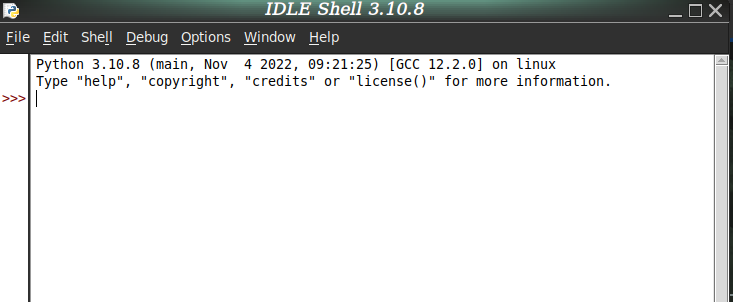
\includegraphics[scale=0.4]{IMG/IDLE-01.png}
\caption{Lancement de l'\textit{IDLE} \texttt{Python}}
\end{center}
\end{figure}
\medskip

A la suite du prompt figuré par les trois chevrons, nous pouvons alors saisir du code \texttt{Python} de façon interactive. L'interface \textit{IDLE} ajoute l'avantage d'afficher les différents éléments syntaxiques dans des couleurs distinctes pour rendre les choses plus lisibles. Une aide contextuelle est aussi fournie.
\medskip

Une autre fonctionnalité intéressante de l'\textit{IDLE} est le rappel des instructions. Les touches \texttt{[Alt] + [p]} (revenir en arrière) et \texttt{[Alt] + [n]} (avancer) permettent de naviguer dans l'historique de saisie des instructions \texttt{Python}.
\medskip

L'\textit{IDLE} \texttt{Python} permet de créer des scripts \texttt{Python} et de travailler directement avec. Pour cela:
\begin{verbatim}
    File  --> New file
\end{verbatim}
\medskip

Une fois votre script enregistré vous pouvez l'exécuter via:
\begin{verbatim}
    Run --> Run Module
\end{verbatim}
\medskip

La sortie apparaît alors dans la fenêtre shell dans l'interpréteur.
\medskip

Pour mieux connaître l'ensemble des fonctionnalités de l'\textit{IDLE} se reporter à la documentation officielle : \url{https://docs.python.org/fr/3/library/idle.html}
\medskip

\subsection*{\texttt{Thonny} un \textit{IDE} pour \texttt{Python}}
\texttt{Thonny} est un \textit{IDE} \texttt{Python} gratuit développé et maintenu par l'Institut d'informatique de l'Université de Tartu, en Estonie. Il s'adresse spécifiquement aux débutants en \texttt{Python}, de sorte que l'interface est simple et épurée et qu'il est facile de la comprendre et de s'y habituer rapidement.
\medskip

Site officiel : \url{https://thonny.org/}
\medskip

\section{Les outils en ligne}
Pour s'exercer à coder depuis n'importe quel ordinateur, où \textit{Python} n'est peut-être pas installé, il est possible de faire appel à des outils en ligne tels que la console interactive du site officiel\footnote{\url{https://www.python.org/shell/}}, \textit{Python Cloud IDE}\footnote{\url{http://pythonfiddle.com/}}, \textit{replit.com}\footnote{\url{www.replit.com}} ou \textit{trinket}\footnote{\url{https://trinket.io/}} qui nous permettent d'écrire du code depuis un navigateur Internet. Si cela peut s'avérer pratique, on ne pourra toutefois pas utiliser des outils avancés.
\medskip

\section{\texttt{Jupyter Notebook}}
\texttt{Jupyter Notebook} est une application \textit{web} qui permet de stocker des lignes de code \texttt{Python}, le résultat de l'exécution du code (notamment des graphiques, tableaux, etc.), ainsi que du texte formaté. Elle offre donc la possibilité d'écrire des petits bouts de code exécutables (insérés dans ce que l'on appelle des \textit{cellules}), de les documenter et d'afficher la résultat de l'exécution. Tout cela est ensuite stocké dans un document partageable. C'est une application fréquemment utilisée par ceux qui travaillent dans l'analyse de données.
\medskip

Installation:
\begin{verbatim}
    # aptitude install jupyter-notebook
\end{verbatim}
\medskip

\texttt{Jupyter Notebook} s'ouvre dans un \textit{navigateur}. Pour créer un \textit{notebook}:
\begin{enumerate}
	\item Cliquer sur \texttt{Nouveau}.
	\item Puis sur \texttt{Python3} (Un nouvel onglet est alors ouvert)
	\item Saisir du code \texttt{Python} dans une \textit{cellule}, puis lancer \texttt{Exécuter}.
\end{enumerate}
\medskip

Il existe quatre types de \textit{cellules}: 
\begin{description}
	\item[\texttt{Code}]: \textit{cellule} qui permet d'insérer du code \texttt{Python}.
	\item[\texttt{Heading}]: type devenu obsolète dans la mesure car avec le type \texttt{markdown} il est beaucoup plus aisé d'insérer des titres.
	\item[\texttt{Text Brut} (pour \texttt{NbConvert}]: permet de contrôler le formatage du document lors d'une conversion du \textit{notebook} en un autre format.
	\item[\texttt{Markdown}]: permet la documentation du \textit{notebook} à l'aide de \textit{balises} \texttt{HTML} ou de la syntaxe \texttt{markdown}\footnote{Pour la syntaxe \texttt{markdown} voir: \url{https://stacklima.com/cellule-markdown-dans-le-bloc-notes- jupyter/}}.
\end{description}
\medskip

\section*{Sources utilisées pour la rédaction de ce chapitre}
\begin{itemize}
	\item[-] \textit{Python Development in Visual Studio Code} (trad. \textit{Développement \textit{Python} avec \texttt{Visual Studio Code}} - Jon \textsc{Fincher} - 4 février 2029 - \url{https://realpython.com/python-development-visual-studio-code/} 
\end{itemize}